% Created 2021-03-27 Sat 14:25
% Intended LaTeX compiler: pdflatex

  \documentclass[english]{article}
  \usepackage[T1, T2A]{fontenc}
\usepackage[lutf8]{luainputenc}
\usepackage[english, russian]{babel}
\usepackage{minted}
\usepackage{graphicx}
\usepackage{longtable}
\usepackage{hyperref}
\usepackage{xcolor}
\usepackage{natbib}
\usepackage{amssymb}
\usepackage{stmaryrd}
\usepackage{amsmath}
\usepackage{caption}
\usepackage{mathtools}
\usepackage{amsthm}
\usepackage{tikz}
\usepackage{grffile}
\usepackage{extarrows}
\usepackage{wrapfig}
\usepackage{rotating}
\usepackage{placeins}
\usepackage[normalem]{ulem}
\usepackage{amsmath}
\usepackage{textcomp}
\usepackage{capt-of}
  
  \usepackage{geometry}
  \geometry{a4paper,left=2.5cm,top=2cm,right=2.5cm,bottom=2cm,marginparsep=7pt, marginparwidth=.6in}
   \usepackage{hyperref}
 \hypersetup{
     colorlinks=true,
     linkcolor=blue,
     filecolor=orange,
     citecolor=black,      
     urlcolor=cyan,
     }

\usetikzlibrary{decorations.markings}
\usetikzlibrary{cd}
\usetikzlibrary{patterns}
\usetikzlibrary{automata, arrows}

\newcommand\addtag{\refstepcounter{equation}\tag{\theequation}}
\newcommand{\eqrefoffset}[1]{\addtocounter{equation}{-#1}(\arabic{equation}\addtocounter{equation}{#1})}


\newcommand{\R}{\mathbb{R}}
\renewcommand{\C}{\mathbb{C}}
\newcommand{\N}{\mathbb{N}}
\newcommand{\rank}{\text{rank}}
\newcommand{\const}{\text{const}}
\newcommand{\grad}{\text{grad}}

\newcommand{\todo}{{\color{red}\fbox{\text{Доделать}}}}
\newcommand{\fixme}{{\color{red}\fbox{\text{Исправить}}}}

\newcounter{propertycnt}
\setcounter{propertycnt}{1}
\newcommand{\beginproperty}{\setcounter{propertycnt}{1}}

\theoremstyle{plain}
\newtheorem{propertyinner}{Свойство}
\newenvironment{property}{
  \renewcommand\thepropertyinner{\arabic{propertycnt}}
  \propertyinner
}{\endpropertyinner\stepcounter{propertycnt}}
\newtheorem{axiom}{Аксиома}
\newtheorem{lemma}{Лемма}
\newtheorem{manuallemmainner}{Лемма}
\newenvironment{manuallemma}[1]{%
  \renewcommand\themanuallemmainner{#1}%
  \manuallemmainner
}{\endmanuallemmainner}

\theoremstyle{remark}
\newtheorem*{remark}{Примечание}
\newtheorem*{solution}{Решение}
\newtheorem{corollary}{Следствие}[theorem]
\newtheorem*{examp}{Пример}
\newtheorem*{observation}{Наблюдение}

\theoremstyle{definition}
\newtheorem{task}{Задача}
\newtheorem{theorem}{Теорема}[section]
\newtheorem*{definition}{Определение}
\newtheorem*{symb}{Обозначение}
\newtheorem{manualtheoreminner}{Теорема}
\newenvironment{manualtheorem}[1]{%
  \renewcommand\themanualtheoreminner{#1}%
  \manualtheoreminner
}{\endmanualtheoreminner}
\captionsetup{justification=centering,margin=2cm}
\newenvironment{colored}[1]{\color{#1}}{}

\tikzset{->-/.style={decoration={
  markings,
  mark=at position .5 with {\arrow{>}}},postaction={decorate}}}
\makeatletter
\newcommand*{\relrelbarsep}{.386ex}
\newcommand*{\relrelbar}{%
  \mathrel{%
    \mathpalette\@relrelbar\relrelbarsep
  }%
}
\newcommand*{\@relrelbar}[2]{%
  \raise#2\hbox to 0pt{$\m@th#1\relbar$\hss}%
  \lower#2\hbox{$\m@th#1\relbar$}%
}
\providecommand*{\rightrightarrowsfill@}{%
  \arrowfill@\relrelbar\relrelbar\rightrightarrows
}
\providecommand*{\leftleftarrowsfill@}{%
  \arrowfill@\leftleftarrows\relrelbar\relrelbar
}
\providecommand*{\xrightrightarrows}[2][]{%
  \ext@arrow 0359\rightrightarrowsfill@{#1}{#2}%
}
\providecommand*{\xleftleftarrows}[2][]{%
  \ext@arrow 3095\leftleftarrowsfill@{#1}{#2}%
}
\makeatother
\author{Ilya Yaroshevskiy}
\date{\today}
\title{Лекция 7}
\hypersetup{
 pdfauthor={Ilya Yaroshevskiy},
 pdftitle={Лекция 7},
 pdfkeywords={},
 pdfsubject={},
 pdfcreator={Emacs 28.0.50 (Org mode )}, 
 pdflang={English}}
\begin{document}

\maketitle
\tableofcontents


\section{Стандартное дискретное распределение}
\label{sec:orgec98cbb}
\subsection{Распределение Бернулли}
\label{sec:org2745e94}
\begin{symb}
\(B_p,\ 0 < p < 1\)
\end{symb}

\begin{definition}
\-
\begin{itemize}
\item \(\xi\) --- число успехов при одном испытии
\item \(p\) --- вероятность успеха при одном испытании
\end{itemize}
\end{definition}
\begin{center}
\begin{tabular}{l|rr}
\(\xi\) & 1 & 0\\
\hline
\(p\) & \(p\) & \(1 - p\)\\
\end{tabular}
\end{center}
\[ E\xi = 0\cdot(1 - p) + 1\cdot p = p \]
\[ D\xi = pq \]
\subsection{Биноминальное распределение}
\label{sec:orga4735ec}
\begin{symb}
\(B_{n,p}\)
\end{symb}
\begin{definition}
\-
\begin{itemize}
\item \(\xi\) --- число успехов при \(n\) испытаниях
\item \(p\) --- вероятность успеха при одном испытании
\end{itemize}
\[ \xi \in B_{n,p} \Leftrightarrow p(\xi = x) = \binom{n}{k}p^k q^{n - k} \]
\end{definition}
\begin{remark}
\(B_p = B_{1, p}\)
\end{remark}
\begin{center}
\begin{tabular}{l|rrllll}
\(\xi\) & 0 & 1 & \(\dots\) & \(k\) & \(\dots\) & \(n\)\\
\hline
\(p\) & \(q^n\) & \(\binom{n}{1}p\cdot q^{n - 1}\) & \(\dots\) & \(\binom{n}{k}p^kq^{n - k}\) & \(\dots\) & \(p^n\)\\
\end{tabular}
\end{center}
\[ \xi =\xi_0 + \xi_1 + \dots + \xi_n \]
, при \(\xi_i \in B_{n, p}\)
\[ E\xi = 0\cdot(1 - p) + 1\cdot p = p \]
\[ D\xi = pq \]
\[ E\xi = \sum_{i = 0}^n E\xi_i = np \]
\[ D\xi = \sum_{i = 0}^n D\xi_i = npq \]
\subsection{Геометрическое распределение}
\label{sec:orgf0493a4}
\begin{symb}
\(G_p\)
\end{symb}
\begin{definition}
\-
\begin{itemize}
\item \(\xi\) --- номер первого успешного испытания
\item \(p\) --- вероятность успеха при одном испытании
\end{itemize}
\[ \xi \ in G_p \Leftrightarrow p(\xi = k) = (1 - p)^{k - 1}\cdot p\quad,1 \le k \le \infty \]
\end{definition}
\begin{center}
\begin{tabular}{l|rrlll}
\(xi\) & 1 & 2 & \(\dots\) & \(k\) & \(\dots\)\\
\hline
\(p\) & \(p\) & \((1 - p )\cdot p\) & \(\dots\) & \((1 - p)^{k - 1}\cdot p\) & \(\dots\)\\
\end{tabular}
\end{center}
\[ E\xi = \sum_{k = 1}^\infty k q^{k - 1}p = p\sum_{k = 0}^\infty (q^k)' = p\left(\sum_{n = 0}^\infty q\right)' = p\cdot\left(\frac{1}{1 - q}\right)' = \frac{1}{p} \]
\[ E\xi^2 = \sum_{k = 1}^p k^2 q^{k - 1} p = p\sum_{k = 1}^\infty\left(k\cdot(k - 1) + k\right)\cdot q^{k - 1} + p\sum_{k = 1}^\infty k\dot q^{k - 1} =  \frac{22q}{p^2} + \frac{1}{p} \]
\[ D\xi = \frac{q}{p^2} \]
\subsection{Распределение Пуассона}
\label{sec:orgde82a06}
\begin{definition}
Слкчайная величина \(\xi\) имеет распределение ПУассона с парметром \(k > 0\), если
\[ p(\xi = k) = \frac{\lambda^k}{k!}e^{-\lambda} \quad, 0\le k < \infty \]
\end{definition}
\begin{center}
\begin{tabular}{l|rrrlll}
\(\xi\) & 0 & 1 & 2 & \(\dots\) & k & \(\dots\)\\
\hline
\(p\) & \(e^{-\lambda}\) & \(\lambda\cdot e^{-\lambda}\) & \(\frac{\lambda^2}{2}\cdot e^{-\lambda}\) & \(\dots\) & \(\frac{\lambda^k}{k!}\cdot e^{-\lambda}\) & \(\dots\)\\
\end{tabular}
\end{center}
\[ E\xi = \lambda \]
\[ E\xi^2 = \lambda^2 + \lambda \]
\[ D\xi = \lambda \]
\[ \simga = \sqrt{\lambda} \]
\subsection{Функция распределения}
\label{sec:org2d27996}
\begin{definition}
\(F\xi(x)\) случайной величины \(\xi\) называется функция
\[ F\xi(x) = p(\xi < x) \]
\end{definition}
\begin{examp}
\begin{center}
\begin{tabular}{l|rr}
\(\xi\) & 0 & 1\\
\hline
\(p\) & 1 - p & p\\
\end{tabular}
\end{center}
\[ F(x) = \begin{cases}
0 & x \le 0 \\
1 - p & 0 < x \le 1
p, x > 1
\end{cases}\]
\end{examp}
\subsubsection{Свойства функции распределения}
\label{sec:orgd3da872}
\begin{property}
\(F(x)\) --- ограниченая функция
\end{property}
\begin{property}
\(F(x)\) --- неубывающая функция
\[ x_1 < x_2 \Rightarrow F(x_1) \le F(x_2) \]
\end{property}
\begin{proof}
\todo
\end{proof}
\begin{property}
\[ p(x_1 \le \xi < x_2) = F(x_2) - F(x_1) \]
\end{property}
\begin{proof}
\todo
\end{proof}

\begin{corollary}
Т.к. Борелевская \(\sigma\)-алгебра порождается интервалами, то зная
функцию распределения можем найти вероятнсоть попадания случайной
величины в любое Борелевское ножество \(B \in \mathfrak{B}\), а
значит полностью задается функцией распределения
\end{corollary}
\begin{property}
\[ \lim_{x \to 0} F(x) = 0 \]
\[ \lim_{x \to + \infty}F(x) = 1 \]
Т.к. функция \(F(x)\) --- ограничена и монотонна, то эти пределы существуют.
\end{property}
\begin{property}
\(x_n \to \pm \infty\)
\[ ] A_n = \{\omega \in \Omega | n - 1\le \xi(\omega) < n\} \]
\[ 1 = p(\Omega) = \sum_{n = 0}^\infty p(A_n) = \sum_{n = 0}^\infty (F(n) - F(n - 1) = \lim_{n \to 0}) = \lim_{N \to 0} \sum_{-N}^N (F(n) - F(n - 1)) = \]
\[ = \lim_{N \to 0} (F(N) - F(-N - 1)) = \lim_{N \to 0}F(N) - \lim_{N \to \infty}F(-N - 1) = 1 \Rightarrow \lim_{N \to \infty} F(N) = 1\]
\todo
\end{property}
\begin{property}
\(F(x)\) --- непрерывна слева, т.е. \(F(x_0 - 0) = F(x_0)\)
\label{orgc8cf814}
\end{property}
\begin{proof}
\-
\begin{itemize}
\item \(] B_n = \{x_0 - \frac{1}{n} \le \xi < x_o\}\)
\end{itemize}
\[ B_0 \supset B_1 \supset \dots \supset B_n \supset \dots \]
\[ \bigcap_{n = 0}^\infty  B_n = \emptyset\]
Следовательно по аксиоме непрерывности
\[\lim_{n \to \infty} p(B_n) = 0 \Rightarrow \lim_{n \to \infty} p(B_n) = \lim_{n \to \infty} (F(x_0) - F(x_0 - \frac{1}{n}) = \]
\[ = F(x_0) - \lim_{n \to \infty} F\left(x_0 - \frac{1}{n}\right) = 0 \]
\[ \lim_{n \to \infty} F\left(x_0 - \frac{1}{n}\right) = F(x_0) \Rightarrow F(x_0 - 0) = F(x_0) \]
\end{proof}
\begin{property}
Скачок в точке \(x_0\) равен вероятности в этой точке.
\[ F(x_0 + 0) - F(x_0) = p(\xi = x_0) \]
\[ \text{или} \]
\[ F(x_0 + 0) = F(x_0) + p(\xi = x_0) = p(\xi \le x_0) \]
\end{property}
\begin{proof}
\-
\begin{itemize}
\item \(C_n = \{x_0 < \xi < x_0 + \frac{1}{n}\}\)
\end{itemize}
По аксиоме непрерывности \(\lim\limits_{n \to \infty} p(C_n) = 0\)
\[ p(C_n) + p(\xi < x_0) = p(\xi = x_0 ) \]
\[ p(x_0 \le \xi < x_0 + \frac{1}{n}) \xrightarrow[n \to \infty]{} p(\xi = x_0) \]
\[ F(x_0 + \frac{1}{n}) - F(x_n) \xrightarrow[n \to \infty]{} p(\xi = x_0) \]
\[ F(x_0 + 0) - F(x_0) = p(\xi = x_0) \]
\end{proof}
\begin{property}
Если \(F(x)\) непрерывна в точке \(x_0\), то \(p(\xi = 0) = 0\). Следствие из \ref{orgc8cf814}
\end{property}
\begin{property}
Если \(F(x)\) непрерывна то, \(p(x_1 \le \xi < x_2) = p(x_1 < \xi < x_2) = p(x_1 \le \xi \le x_2) = p(x_1 < \xi \le x_2) = F(x_2) - F(x_1)\)
\end{property}
\begin{property}
Случайная величина \(\xi\) имеет дискретное распредление \(\Leftrightarrow\) ее функция распределения -- ступенчатая функция 
\end{property}
\section{Абсолютно непрерывные случайные величины}
\label{sec:org400ccbd}
\begin{definition}
Случайная величина \(\xi\) имеет \textbf{абсолютно непрерывное} распределение, если для любового Борелевского множества \(B \in \mathfrak{B}\)
\[ p(\xi \in B) = \int\limits_B f_\xi(x) dx \]
для некоторой функции \(f_\xi(x)\). Интеграл Лебега а не Римана.
\end{definition}
\begin{definition}
\(f_\xi(x)\) --- \textbf{плотность распределения} случайной величины \(\xi\)
\end{definition}
\subsection{Свойства плотности и функции распределения}
\label{sec:orgac852dd}
\beginproperty
\begin{property}
\textbf{Вероятностный геометрический} смысл плотности.
\[ p(\alpha < \xi < \beta) = \int\limits_\alpha^\beta f_\xi(x) dx \]
\begin{center}
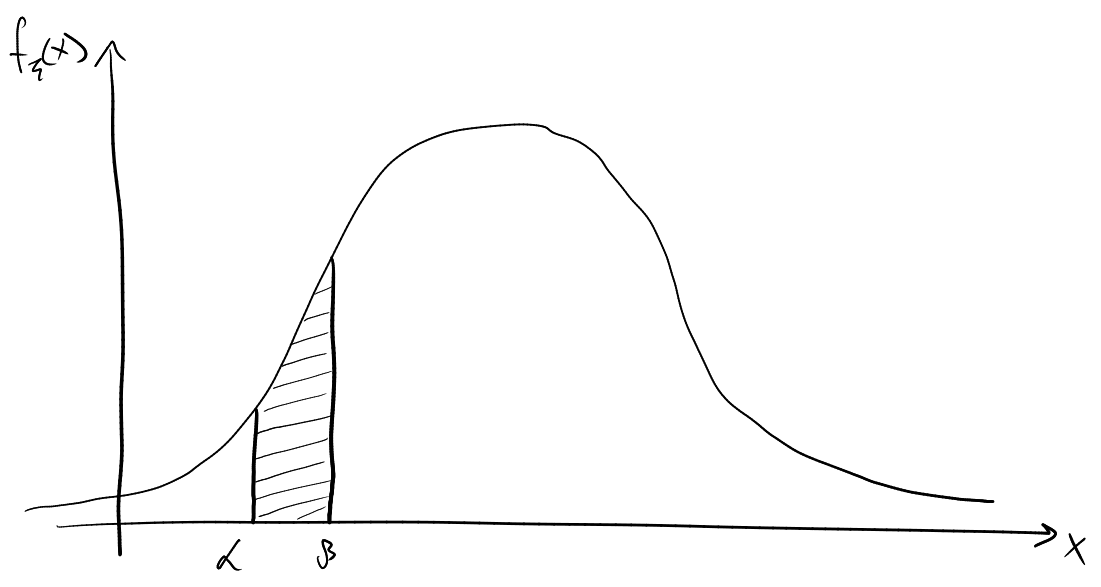
\includegraphics[scale=0.3]{7_1.png}
\end{center}
\[ S = p(\alpha < \xi < \beta) \]
\end{property}
\begin{proof}
Из определения распределения \(B = (\alpha, \beta)\)
\end{proof}
\begin{property}
\textbf{Условие нормировки}
\[ \int\limits_{-\infty}^{+ \infty} f(x) dx = 1 \]
\label{orgcdb42a6}
\end{property}
\begin{proof}
По определению \(p(\xi \in \R) = 1\) а \(B = \R \in \mathfrak{B}\) \fixme
\end{proof}
\begin{property}


\[ F\xi(x) = \int\limits_{- \infty}^{+\infty} f(x) dx\]
\end{property}
\begin{proof}
По поределению
\[ F_\xi(x) = p(\xi < x) = \int_{-\infty}^x  f(x) dx \quad B = (-\infty, x)\]
\end{proof}
\begin{property}
\(F_\xi(x)\) --- непрерывная функция. Как интеграл с переменным верхним пределом
\end{property}
\begin{property}
\(F_\xi(x)\) --- дифференцируема почти всюду и
\[ f_\xi(x) = F'(x) \]
почти для всех \(x\)
\label{org801551d}
\end{property}
\begin{proof}
Теорема Барроу.
\end{proof}
\begin{remark}
Почти для всех, кроме возможно \(x\) из множества нулевой меры Лебега.
\end{remark}
\begin{property}
\(f_\xi(x) > 0\)
\label{orgd37bd39}
\end{property}
\begin{proof}
Из определения или из \ref{org801551d}
\end{proof}
\begin{property}
\(p(\xi = x_0) = 0\)
\end{property}
\begin{property}
\(p(x_1 </\le \xi </\le x_2) = F(x_2) - f(x_1)\)
\end{property}
\begin{property}
Если для \(f(x)\) выолнено свойства \ref{orgcdb42a6} и \ref{orgd37bd39} то она является плотностью некоторой случайной величины
\end{property}
\subsection{Числовые характеричтики}
\label{sec:org22f00be}
\begin{definition}
\textbf{Математическим ожиданием} абсолютно непрерывной случайной величины \(\xi\) называется число
\[ E\xi = \int\limits_{- \infty}^{+\infty} x f(x) dx \]
при условии что данный интеграл сходится абсолютно, т.е. \(\int\limits_{- \infty}^{ + \infty} |x| f(x) dx < \infty\)
\end{definition}
\begin{definition}
\textbf{Дисперсией} абсолютно непрерывной случайной величины \(\xi\) называется число
\[ D\xi = E(\xi - E\xi) = \int\limits_{- \infty}^{ + \infty}(x - E\xi)^2 f(x) dx \]
при условии что интеграл сходится абсолютно
\end{definition}
\begin{remark}
\[ D\xi = E\xi^2 - (E\xi)^2 = \int\limits_{-\infty}^{ + \infty}x^2 f(x) dx - (E\xi)^2 \]
\end{remark}
\begin{definition}
\textbf{Среднее квадратическое отклонение} \(\sigma_\xi = \sqrt{D\xi}\)
\end{definition}
\begin{remark}
Смысл свойств этих числовых характеристик полоностью идентичны дискретной случайной величины
\end{remark}
\end{document}
